\documentclass[10pt]{article}
\usepackage{amsmath,amsfonts,times}
\usepackage{graphicx,color,tikz}
\usepackage[paperwidth=17.6cm,paperheight=10.2cm,lmargin=0in,rmargin=0in,tmargin=0.in,bmargin=0.in]{geometry}
\usepackage{bm}
\usetikzlibrary{arrows.meta,shadows,positioning,calc,backgrounds}

% One color per primitive type, and one for operations.
\definecolor{cbox}{rgb}{0.10,0.35,0.80}
\definecolor{cball}{rgb}{0.05,0.55,0.20}
\definecolor{ccyl}{rgb}{0.80,0.10,0.10}
\definecolor{cop}{rgb}{0.50,0.20,0.65}

\tikzset{
  node/.style={draw=black, minimum width=11mm, minimum height=7mm, rectangle, very thick, fill=white, drop shadow, rounded corners=4pt, font=\small},
  leaf/.style={node, minimum width=13mm},
  edge/.style={thick, draw=black},
  order/.style={circle, draw=black, fill=yellow!40, inner sep=1pt, minimum width=4.6mm, font=\scriptsize\bfseries},
  slot/.style={draw=black, thick, minimum width=13mm, minimum height=5.2mm, inner sep=1pt, font=\scriptsize, fill=white},
  arr/.style={draw=black, thick, minimum width=14mm, minimum height=5.2mm, inner sep=1pt, font=\scriptsize},
  head/.style={font=\small\bfseries, anchor=west},
}

\begin{document}
\nopagecolor
\centering
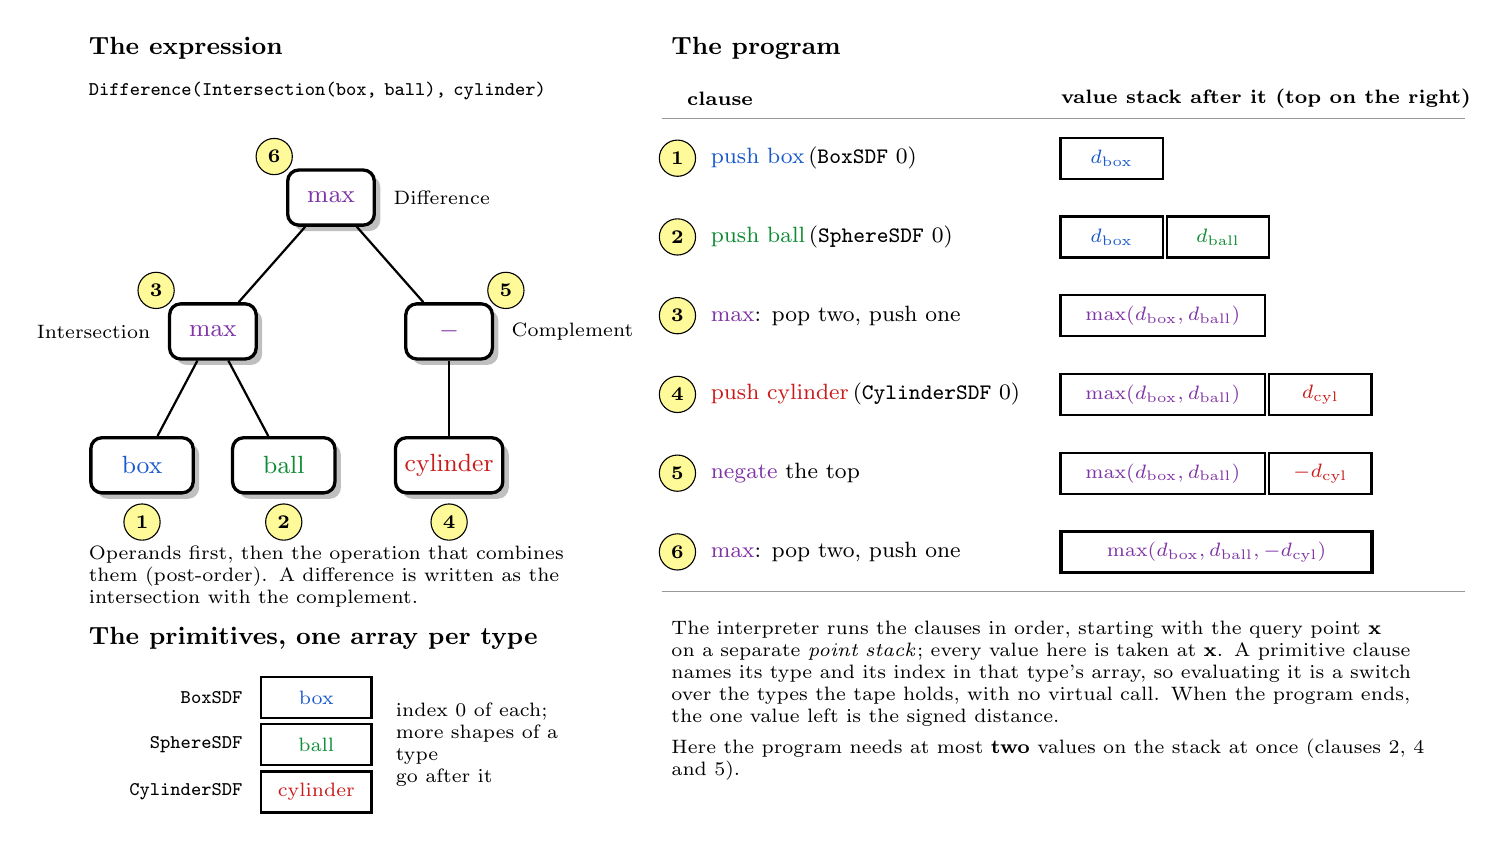
\begin{tikzpicture}[x=1cm, y=1cm]

  % ── The expression, as the builder makes it: Difference(a, b) is Intersection(a, Complement(b)).
  \node[head] at (-0.2,9.7) {The expression};
  \node[font=\scriptsize, anchor=west, text width=7.2cm] at (-0.2,9.15) {\texttt{Difference(Intersection(box, ball), cylinder)}};

  \node[node, text=cop] (R)  at (3.0,7.8) {$\max$};
  \node[node, text=cop] (I)  at (1.5,6.1) {$\max$};
  \node[node, text=cop] (C)  at (4.5,6.1) {$-$};
  \node[leaf, text=cbox]  (A)  at (0.6,4.4) {box};
  \node[leaf, text=cball] (B)  at (2.4,4.4) {ball};
  \node[leaf, text=ccyl]  (Y)  at (4.5,4.4) {cylinder};

  \draw[edge] (R) -- (I);
  \draw[edge] (R) -- (C);
  \draw[edge] (I) -- (A);
  \draw[edge] (I) -- (B);
  \draw[edge] (C) -- (Y);

  \node[font=\scriptsize, anchor=west] at ($(R.east)+(0.1,0)$) {Difference};
  \node[font=\scriptsize, anchor=east] at ($(I.west)+(-0.1,0)$) {Intersection};
  \node[font=\scriptsize, anchor=west] at ($(C.east)+(0.1,0)$) {Complement};

  % Post-order: the order the clauses are written in.
  \node[order] at ($(A.south)+(0,-0.35)$) {1};
  \node[order] at ($(B.south)+(0,-0.35)$) {2};
  \node[order] at ($(I.north west)+(-0.15,0.15)$) {3};
  \node[order] at ($(Y.south)+(0,-0.35)$) {4};
  \node[order] at ($(C.north east)+(0.15,0.15)$) {5};
  \node[order] at ($(R.north west)+(-0.15,0.15)$) {6};

  \node[font=\scriptsize, anchor=north west, text width=6.4cm, align=left] at (-0.2,3.5) {%
    Operands first, then the operation that combines them (post-order). A difference is written as the
    intersection with the complement.};

  % ── The primitive arrays: one per type, in the tape's pool.
  \node[head] at (-0.2,2.2) {The primitives, one array per type};
  \node[font=\scriptsize, anchor=east] at (2.0,1.45) {\texttt{BoxSDF}};
  \node[arr, text=cbox, anchor=west] at (2.1,1.45) {box};
  \node[font=\scriptsize, anchor=east] at (2.0,0.85) {\texttt{SphereSDF}};
  \node[arr, text=cball, anchor=west] at (2.1,0.85) {ball};
  \node[font=\scriptsize, anchor=east] at (2.0,0.25) {\texttt{CylinderSDF}};
  \node[arr, text=ccyl, anchor=west] at (2.1,0.25) {cylinder};
  \node[font=\scriptsize, anchor=west, text width=2.6cm, align=left] at (3.7,0.85) {index 0 of each;\\ more shapes of a type\\ go after it};

  % ── The program: one clause per node, and the value stack after each.
  \begin{scope}[shift={(7.4,0)}]
    \node[head] at (-0.2,9.7) {The program};
    \node[font=\scriptsize\bfseries, anchor=west] at (0.0,9.05) {clause};
    \node[font=\scriptsize\bfseries, anchor=west] at (4.75,9.05) {value stack after it (top on the right)};
    \draw[black!40] (-0.2,8.8) -- (10.0,8.8);

    % Row y positions.
    \foreach \i/\y in {1/8.3, 2/7.3, 3/6.3, 4/5.3, 5/4.3, 6/3.3} {
      \node[order] at (-0.0,\y) {\i};
    }

    \node[anchor=west, font=\footnotesize] at (0.3,8.3) {\textcolor{cbox}{push box}\,(\texttt{BoxSDF} 0)};
    \node[anchor=west, font=\footnotesize] at (0.3,7.3) {\textcolor{cball}{push ball}\,(\texttt{SphereSDF} 0)};
    \node[anchor=west, font=\footnotesize] at (0.3,6.3) {\textcolor{cop}{max}: pop two, push one};
    \node[anchor=west, font=\footnotesize] at (0.3,5.3) {\textcolor{ccyl}{push cylinder}\,(\texttt{CylinderSDF} 0)};
    \node[anchor=west, font=\footnotesize] at (0.3,4.3) {\textcolor{cop}{negate} the top};
    \node[anchor=west, font=\footnotesize] at (0.3,3.3) {\textcolor{cop}{max}: pop two, push one};

    % Stacks.
    \node[slot, anchor=west, text=cbox] at (4.85,8.3) {$d_\text{box}$};

    \node[slot, anchor=west, text=cbox] at (4.85,7.3) {$d_\text{box}$};
    \node[slot, anchor=west, text=cball] at (6.2,7.3) {$d_\text{ball}$};

    \node[slot, anchor=west, text=cop, minimum width=26mm] at (4.85,6.3) {$\max(d_\text{box}, d_\text{ball})$};

    \node[slot, anchor=west, text=cop, minimum width=26mm] at (4.85,5.3) {$\max(d_\text{box}, d_\text{ball})$};
    \node[slot, anchor=west, text=ccyl] at (7.5,5.3) {$d_\text{cyl}$};

    \node[slot, anchor=west, text=cop, minimum width=26mm] at (4.85,4.3) {$\max(d_\text{box}, d_\text{ball})$};
    \node[slot, anchor=west, text=ccyl] at (7.5,4.3) {$-d_\text{cyl}$};

    \node[slot, anchor=west, text=cop, very thick, minimum width=39.5mm] at (4.85,3.3) {$\max(d_\text{box}, d_\text{ball}, -d_\text{cyl})$};

    \draw[black!40] (-0.2,2.8) -- (10.0,2.8);

    \node[anchor=north west, font=\scriptsize, text width=9.6cm, align=left] at (-0.2,2.55) {%
      The interpreter runs the clauses in order, starting with the query point $\mathbf{x}$ on a separate
      \emph{point stack}; every value here is taken at $\mathbf{x}$. A primitive clause names its type and its
      index in that type's array, so evaluating it is a switch over the types the tape holds, with no virtual call.
      When the program ends, the one value left is the signed distance.\\[3pt]
      Here the program needs at most \textbf{two} values on the stack at once (clauses 2, 4 and 5).%
    };
  \end{scope}

\end{tikzpicture}

\end{document}
